\section{Mathematical Foundations}
\label{sec:math-foundations}
This section serves as a short introduction to the mathematical concepts used throughout this paper.
For the basic concepts of measure theory such as sigma algebras and measures, which will be necessary for understanding the derivations of the metrics in this section, we refer to the textbook by \citeasnoun{Elstrodt2007}.
For a comprehensive overview on stochastic programming, see \citeasnoun{Birge1997}.
Concerning probability theory, nothing beyond the basic definitions is used.
Any introductory text such as \citeasnoun{Billingsley1995} or \citeasnoun{Bauer1991} should suffice.
In section \ref{sec:expect-max-algos}, some concepts from machine learning are used.
To the reader unfamiliar with these concepts, the recent textbook by \citeasnoun{Bishop2006} is highly recommended.

This section is organized as follows.
First, the notation and basic definitions used in this thesis are introduced.
The discussion starts with an introduction to the relationship of stochastic programming problems and scenario trees\footnote{The term scenario tree is used colloquially at first. In the following section, a rigorous definition will be given.}.
Then, the Kantorovich distance is introduced as a metric for measuring the discretization quality of a scenario tree.
Finally, this metric is used to formalize the problem of optimal scenario tree generation.
\subsection{Notation and Definitions}
In this section, the most often used mathematical objects are defined.
The definitions generally used for random variables and stochastic processes are very broad.
For the purposes of this paper, the following narrower definitions will suffice.
The narrow definitions will allow for shorter and more coherent theorems and statements.
This is not to say that the algorithms presented in this paper are not applicable to a more general set of problems.
The purpose of this thesis is not, however, to derive the most general theorems, but instead to provide a good understanding of the novel ideas developed in sections \ref{sec:two-theorems} and \ref{sec:expect-max-algos}.
\begin{definition}[Random Variable]
  \label{def:random_variable}
  Let $(\Omega, \mathfrak{A}, \mathbb{P})$ a probability space.
  Let $\bs\zeta$ be a mapping $\bs\zeta:\Omega\rightarrow\mathbb{R}^d$, which is $\mathfrak{A}$-measurable.
  Then, $\bs\zeta$ is called a \textbf{random variable}.
  If $|\Omega|<\infty$, $\bs\zeta$ is called a \textbf{discrete random variable}.
  \end{definition}
\begin{remark}
  Throughout this thesis, random objects will be printed as bold characters, while their realizations (mappings) will be denoted by the same symbol in normal face.
  %For example, for the discrete random variable $\bs\zeta$, this means $\bs\zeta(\omega_i) = \zeta_i$.
\end{remark}
\begin{remark}[Notation for discrete random variables]
  \label{remark:discrete-randvar-indexsets}
  Consider a discrete random variable $\bs\zeta$.
  Without loss of generality, we will assume that $\mathfrak{P}(\Omega)$ generates $\mathfrak{A}$.
  The $\sigma$-algebra is therefore always implicit in the set of events.
  For a discrete random variable $\bs\zeta$, since $|\Omega|=N<\infty$, there exists a bijective mapping $\phi$ and a set $I=\{1,\ldots, N\}$ such that $\phi:\Omega \rightarrow I$.
  Using this mapping, we denote $\zeta_i := \zeta(\phi^{-1}(i))\,\forall\,i\in I$.
  For easier reading, the probability distributions of general random variables are denoted by upper case bold face characters $\mathbb{P,Q}$, while for discrete random variables lower case letters $p$ and $q$ are used.
  Similar to the events, define $p_i := p(\phi^{-1}(i))\,\forall\,i\in I$.
\end{remark}
\begin{definition}[Stochastic Process]
\label{def:stochastic_process}
  Let $\bs\xi:=\{\bs\zeta^t\}_{t=1}^T,\; t=1..T,\, T\in\mathbb{N}$ be a sequence of random variables $\bs\zeta^t$ with corresponding probability spaces $(\Omega, \mathfrak{A}_t, \mathbb{P}_t)$.
  If the sequence of sigma algebras $\mathcal{F}:=\{\mathfrak{A}_t\}_{t=1}^T$ is monotone, meaning $\mathfrak{A}_1\subset\mathfrak{A}_2\subset\ldots\subset\mathfrak{A}_T$, then $\bs\xi$ is a \textbf{stochastic process}.
  $\mathcal{F}$ is called the \textbf{filtration} of $\bs\xi$.
  If $|\Omega|<\infty$, $\xi$ is called a \textbf{discrete stochastic process}.
  The events $\omega\in\Omega$ of a discrete stochastic process are called \textbf{scenarios}.
\end{definition}
\begin{remark}
  \label{remark:stochproc-as-randvar}
  Stochastic processes can be considered in terms of random variables by the following transformation.
  Let $\bs\xi = \{\bs\zeta^t\}_{t=1}^T$ be a stochastic process.
  Consider the random variable $\bs\chi$ that is defined by the probability space $(\Omega, \mathfrak{A}_T, \mathbb{P}_T)$ and the mapping \[\chi:\Omega\rightarrow \mathbb{R}^{T\times d},\,\omega\mapsto\left[\begin{array}{c}\zeta^1(\omega)\\\vdots\\\zeta^T(\omega)\end{array}\right].\]
  $\bs\chi$ will be denoted as the random variable \textbf{induced} by $\bs\xi$.
  Note that this transformation discards the filtration information.

  The notational conventions introduced in remark \ref{remark:discrete-randvar-indexsets} apply accordingly to discrete stochastic processes.
  The term `stochastic process' may be abbreviated by SP.
\end{remark}
\begin{remark}[Notation of SPs]
In this work, only stochastic processes with discrete time steps will be considered.
These time steps will be indexed from 1 to a final time $T$.
For a stochastic process $\bs\xi$ with a continuous distribution, $\xi^t$ denotes the mapping from events to outcomes at time step $t$.
For discrete stochastic processes, index sets for the events, typically denoted by $I$ and $J$, are introduced.
The outcome of an event $i\in I$ of a discrete stochastic process $\bs\xi$ at time step $t$ is denoted by $\xi_i^t$.
If the time step is omitted, this denotes the full scenario $i$, that is the vector of the values $\xi_i^t$ sorted by their times $t$.
\end{remark}
\begin{remark}[Probability densities and distributions]
  In this thesis, the liberal approach of \citeasnoun{Bishop2006} with respect to the terms probability density and probability distribution will be used.
The term distribution will be used throughout to mean both.
Given an event space $\Omega$, a $\sigma$-algebra $\mathfrak{A}$, and a continuous distribution $\mathbb{P}$, $\mathbb{P}(\omega)$ for $\omega\in\Omega$ will denote the value of the underlying probability density, while $\mathbb{P}(A)$ for $A\in\mathfrak{A}$ will denote the value of the distribution.
Though this notation may seem unclear, the meaning will always be obvious.
On the other hand, by avoiding the proliferation of additional symbols, the notation achieves greater clarity.
\end{remark}
The vector $e$ denotes a vector of ones in each dimension.
The dimension will be chosen in accordance with the context.

In optimization problems, if there are indices in an equation that are not explicitly declared, it is assumed that this equation is stated for each of the indices in the corresponding set.
The corresponding set will always be obvious in context.
\subsection{Stochastic Programming and Scenario Trees}
Consider the following multi-stage stochastic programming problem
\begin{subequations}
  \label{eq:genericSP}
\begin{eqnarray}
  \mathcal{P}(\hat{\bs\xi})\;\min_{\hat{\bs x}} &&\mathbb{E}\left[\sum_{t=1}^Tf_t(\hat{\bs\xi}^t, \hat{\bs x}^t)\right]\\
  &\mathrm{s.t.}& h_t(\hat{\bs\xi}^t, \hat{\bs x}^t, \hat{\bs x}^{t-1}) = 0\\
  &&\hat{\bs x}^t \in X_t\\
  &&\hat{\bs x}^t \, \mathrm{is}\,\mathfrak{A}_t \mathrm{-measurable} \label{eqn:measurability-constraint}
\end{eqnarray}
\end{subequations}
governed by a stochastic process $\hat{\bs\xi}(\Omega, \mathcal{F}, \mathbb{P}_t),\;\hat{\bs\xi}^t : \Omega\rightarrow\mathbb{R}^{d_1}$.
Note that the solution $\hat{\bs x}$ to this problem is a stochastic process $\hat{\bs x}(\Omega, \mathcal{F}, \mathbb{P}_t),\;\hat{\bs x}^t : \Omega\rightarrow\mathbb{R}^{d_2}$ over the same probability space.

The difficulty in multi-stage stochastic programming problems arises from the measurability constraint (\ref{eqn:measurability-constraint}).
This constraint is specific to multi-stage stochastic programs and leads to a much increased computational complexity of multi-stage programs over two-stage programs \cite{Shapiro2005,Shapiro2008}.
%
\paragraph{Measurability Constraints}
The measurability constraints imply that the condition
\begin{equation}
  \label{eq:mathematical-NAC}
  \omega_1,\omega_2\in \Omega \, : \, \hat{\xi}^\tau(\omega_1) = \hat{\xi}^\tau(\omega_2)\,\forall \tau\leq t\,\Rightarrow \,  \hat{x}^t(\omega_1) =  \hat{x}^t(\omega_2)
\end{equation}
has to hold for all time steps $t$, and all pairs of events $(\omega_1,\omega_2)\in\Omega^2$.
Note that this implies that the decision variables $\hat{\bs x}^t$ must only depend on the events of the past up until the present $\hat{\bs\xi}^1$, ..., $\hat{\bs\xi}^t$, and explicitly \textbf{not} on $\hat{\bs\xi}^{t+1},\, ...,\,\hat{\bs\xi}^T$.
This property is called \textit{non-anticipativity of the solution} $\hat{\bs x}$.
These equations model the uncertainty of the future.
%
\paragraph{Discretization}
%
Stochastic programs are infinite dimensional optimization problems and as such not immediately accessible to computation.
To transform the stochastic program into a computable problem, the infinite dimensional stochastic process $\hat{\bs\xi}$ must be discretized into a finite stochastic process $\bs\xi$ (see figure \ref{fig:abstract-discretization}).

If certain precautions are taken, it is possible to show (at least for linear stochastic programs) that the solution to the stochastic problem is stable under this discretization operation, meaning that there exists a factor $L$ such that the distance between the solution to the discretized problem $\bs x$ and the solution to the original problem $\hat{\bs x}$ are Lipschitz-continuous with respect to the discretization error:
\begin{equation}
  D(\bs x , \hat{\bs x}) \leq L\cdot D(\bs\xi,\hat{\bs\xi})
\end{equation}
where $D$ is an appropriate metric. See \citeasnoun{Heitsch2010} for the proof and further details.
%The correct choice for $D$ will be discussed in sections \ref{sec:measuring-challenges} and \ref{sec:kantoro}.
\pgfdeclarelayer{background}
\pgfsetlayers{background,main}
\begin{figure}
  \centering
    \begin{tikzpicture}[node distance=5cm, auto]
      \node [block] (xiorig) {$\xi$};
      \node [block, below of=xiorig] (xi) {$\hat{\xi}$};
      \node [block, text width=10em, right of=xiorig] (infsolver){Infinite Dim. Solver};
      \node [block, right of=infsolver] (xorig){$x$};
      \node [block, text width=10em, below of=infsolver] (nlp) {(N)LP Solver};
      \node [block, below of=xorig] (x) {$\hat{x}$};

      \path [line] (xiorig) -- node (xierror) {$D(\xi,\hat{\xi})$} (xi);
      \path [line] (x) -- node (xerror) {$D(x,\hat{x})$} (xorig);
      \path [line,dashed] (xierror) -- node {$L\cdot D(\xi,\hat{\xi})\geq D(x,\hat{x})$} (xerror);
      \path [line] (xiorig) -- (infsolver);
      \path [line] (xi) -- (nlp);
      \path [line] (nlp) -- (x);
      \path [line] (infsolver) -- (xorig);

      \node [node distance=1.4cm,below of=xi] (focus){Focus of this paper};
      \begin{pgfonlayer}{background}
        \node (selection) [draw, rounded corners,dotted, fill=orange!20, fit=(xiorig) (xi) (xierror) (focus)] {};
      \end{pgfonlayer}
    \end{tikzpicture}
  \caption{Steps in the discretization of a stochastic program. Since the infinite dimensional solver is just a theoretical enitiy, The path below must be used. A discretization error is introduced when converting $\xi$ to $\hat{\xi}$. This error is propagated through the NLP. For linear stochastic programs, it has been shown %Heitsch2010
    that there exists a problem specific constant $L$ such that the error between the discretized and the original solution is bounded by the error in the discretization of the stochastic process.}
  \label{fig:abstract-discretization}
\end{figure}

%%% Local Variables: 
%%% mode: latex
%%% TeX-master: "da"
%%% End: 

The discretization will be carried out in two steps.
First, the infinite dimensional stochastic process $\hat{\bs\xi}$ is approximated by a discrete stochastic process $\bs\xi(I,\mathcal{F},p)$ defined by a set of scenarios $\{\xi_i, i\in I\}$  sampled using Monte-Carlo techniques.
This step is well known and will not be discussed here.
To capture the essence of the non-anticipativity constraints, in a second step the scenarios of $\bs\xi$ are recombined into a tree structure.
Tree structures play a central role in this work.
For completeness, we will define the basic notions used here in the following definition.
For a complete overview over the graph theoretical terms, see for example \citeasnoun{Diestel2005}.
\begin{definition}[Tree \cite{Diestel2005}]
  \label{def:tree}
  An acyclic, connected Graph is called a \textbf{tree}.
  The nodes of a tree with degree 1 are called \textbf{leafs}.
  A tree, in which one node is designated as the \textbf{root node} is called a \textbf{rooted tree}.
\end{definition}
There exists a natural relationship between discrete stochastic processes and rooted trees.
\begin{definition}[Filtration Tree]
  \label{def:filtration_tree}
  Let $\bs\xi$ be a discrete stochastic process $\bs\xi(\Omega, \mathcal{F}, p)$.
  Let $\mathcal{T}$ be a rooted tree with a set $\mathcal{N}$ of nodes, such that each the path from each leaf node to the root node has the same length.
  Let $\mathcal{N}_t$ be the set of nodes of $\mathcal{T}$ at depth $t$.
  For every time step $t$, let $\mathfrak{E}_t$ be the (unique) disjoint cover of $\Omega$, such that $\mathcal{F}_t$ is the sigma-algebra generated by $\mathfrak{E}_t$.
  If there exists a family of mappings $\phi_t:\mathfrak{E}_t\rightarrow \mathcal{N}_t$, such that
  \begin{enumerate}
  \item  $\forall\, e_1,e_2\subset \Omega$ with $e_1\in\mathfrak{E}_t$, $e_2\in\mathfrak{E}_{t+1}$ and $e_2\subset e_1\;\Rightarrow\;\phi_t(e_1)$ is the parent node of $\phi_{t+1}(e_2)$.
  \item $\phi_t$ is bijective.
  \end{enumerate}
  Then, $\mathcal{T}$ is called the \textbf{filtration tree} of $\mathcal{F}$.
\end{definition}
\begin{remark}[Nodes and scenarios]
  Given a filtration tree, there exists a mapping $n$ that maps a scenario index and a time step to the corresponding node:
  \begin{equation}
    \label{eq:71}
    n:I\times \{1,\ldots T\}\rightarrow\mathcal{N}
  \end{equation}
  This mapping will be used extensively for the derivation of the algorithms.
  In an abuse of notation, we will denote the set of all pairs of scenarios and the time step t corresponding to the node $k$ by $n^{(-1)}(k)$.
\end{remark}
The filtration tree is the basis for the scenario tree defined in the following.
\begin{definition}[Scenario Tree]
  Let a discrete stochastic process $\bs\xi$ and a corresponding filtration tree $\mathcal{T}$ be given as above.
  Using the bijective mappings $\phi_t$ from definition \ref{def:filtration_tree}, a mapping of node values
  \[
  \nu:\mathcal{N}\rightarrow\mathbb{R}^d,\; n\mapsto \bs\xi(\phi_t^{-1}(n))
  \]
  where $t$ is chosen according to the depth of $n$,
  and a mapping of probabilities
  \[
  q:\mathcal{N}_T\rightarrow\mathbb{R},\; n\mapsto p(\phi_T^{-1}(n))
  \]
  can be constructed.
  The triple $(\mathcal{T}, \nu, q)$ is called a \textbf{scenario tree}.
\end{definition}
Neglecting symmetric solutions, there exists a bijective mapping between discrete stochastic processes and scenario trees.
Due to this identity, the terms scenario tree and discrete stochastic process will be used interchangeably where appropriate, and both objects will be denoted by the same symbol.
\begin{remark}[Node values and scenario values]
The mapping $\nu$ of nodes to node values can be represented by a finite vector.
Using the filtration tree, the values of the scenarios at each time step can be can be represented by the node values.
The value of scenario $i$ at time step $t$ will be denoted by $\nu_i^t$. To make the distinction between node values and scenario values, the following convention is used: Subscripts $i$ and $j$ correspond to scenario values, while the subscript $n$ corresponds to node values.
\end{remark}

Tree structures introduce the non-anticipativity constraints in intuitive way (see figure \ref{fig:violated-nonanticipativity}).
The parent node holds the information of the past, while each node is branched into multiple possible future states.
It is a common mistake to represent the stochastic process as a set of independent scenarios with common root.
Because this is a common misconception, for illustration purposes we will give the following
\begin{example}[Necessity of tree structure]
  \label{ex:tree-necessity}
  % \hangindent=1cm
  Consider a game of coin tosses, played by a player against a bank.
  The player will play the game for three consecutive coin tosses.
  He has three Euros that he wants to wager.
  Predicting the outcome of the toss correctly will return
  \begin{itemize}
  \item $\frac{13}{6}$ the stakes $x$ in the first round,
  \item $2\cdot x$ in the second round,
  \item and only $1.5\cdot x$ in the final round.
  \end{itemize}
  Otherwise the stakes will be lost.
  Earnings cannot be used again as wager.

  The player optimizes the expected return.
  Without the need for a calculator we can say that the optimal strategy is to bet everything in the first round, yielding a total expected return of $1.75$.

  Consider now a transcription of the problem as an LP, using all possible scenarios (see figure \ref{fig:violated-nonanticipativity}, top).
  For three consecutive coin tosses, there are eight different scenarios.
  The player wants to use this LP to help him decide how much he is supposed to bet in the first round.
  The corresponding LP is
  \begin{align*}
    \min\limits_x &\; \sum_{i\in I}\sum_{t=1}^3p_ix_i^t \xi_i^t\\
    \text{s.t.} &\; \sum_{t=1}^3x_i^t = 3 \\
    & \; x_i^1 = x_0^1
  \end{align*}
  where $I$ is the index set of scenarios, $\xi_i^t$ is the outcome of the game (return per Euro for win, $0$ for loss), $x_i^t$ is the amount that the player is willing to bet at time step $t$ in scenario $i$. The first equation ensures that the player spends exactly the amount he has at his disposal. The second equation fixes the players decision in the first round.

  The results, summarized in table \ref{tab:coin-toss-results}, show that the solution of the LP does not match the optimal solution, even though the uncertainty was seemingly taken into account.
  The flaw in the above formulation is that the non-anticipativity constraints are missing for stage 2.
  The algorithm believes to know what will happen, as soon as the first value is revealed.
  The game, as it is modeled in the LP is as follows:
  ``Make one decision with stochastic outcome, then make two decisions with perfect foresight''.
  In this situation, the algorithm will decide to wait and only wager, when the result is (seemingly) known beforehand (see figure \ref{fig:violated-nonanticipativity}).
  \begin{figure}
  \centering
    \begin{tikzpicture}
      \node (root) at (0,0) [circle,draw] {$x_{\mathrm{now}}$};
      \node (n11) at (2,3.5) [circle,draw]  {W};
      \node (n12) at (2,2.5) [circle,draw]  {W};
      \node (n13) at (2,1.5) [circle,draw]  {W};
      \node (n14) at (2,0.5) [circle,draw]  {W};
      \node (n18) at (2,-3.5) [circle,draw] {L};
      \node (n17) at (2,-2.5) [circle,draw] {L};
      \node (n16) at (2,-1.5) [circle,draw] {L};
      \node (n15) at (2,-0.5) [circle,draw] {L};

      \node (n21) at (4,3.5) [circle,draw]  {$x_{11}$};
      \node (n22) at (4,2.5) [circle,draw]  {$x_{12}$};
      \node (n23) at (4,1.5) [circle,draw]  {$x_{13}$};
      \node (n24) at (4,0.5) [circle,draw]  {$x_{14}$};
      \node (n28) at (4,-3.5) [circle,draw] {$x_{18}$};
      \node (n27) at (4,-2.5) [circle,draw] {$x_{17}$};
      \node (n26) at (4,-1.5) [circle,draw] {$x_{16}$};
      \node (n25) at (4,-0.5) [circle,draw] {$x_{15}$};

      \node (n31) at (6,3.5) [circle,draw]  {W};
      \node (n32) at (6,2.5) [circle,draw]  {W};
      \node (n33) at (6,1.5) [circle,draw]  {L};
      \node (n34) at (6,0.5) [circle,draw]  {L};
      \node (n38) at (6,-3.5) [circle,draw] {L};
      \node (n37) at (6,-2.5) [circle,draw] {L};
      \node (n36) at (6,-1.5) [circle,draw] {W};
      \node (n35) at (6,-0.5) [circle,draw] {W};

      \node (n41) at (8,3.5) [circle,draw]  {$x_{21}$};
      \node (n42) at (8,2.5) [circle,draw]  {$x_{22}$};
      \node (n43) at (8,1.5) [circle,draw]  {$x_{23}$};
      \node (n44) at (8,0.5) [circle,draw]  {$x_{24}$};
      \node (n48) at (8,-3.5) [circle,draw] {$x_{28}$};
      \node (n47) at (8,-2.5) [circle,draw] {$x_{27}$};
      \node (n46) at (8,-1.5) [circle,draw] {$x_{26}$};
      \node (n45) at (8,-0.5) [circle,draw] {$x_{25}$};

      \node (n51) at (10,3.5) [circle,draw]  {W};
      \node (n52) at (10,2.5) [circle,draw]  {L};
      \node (n53) at (10,1.5) [circle,draw]  {W};
      \node (n54) at (10,0.5) [circle,draw]  {L};
      \node (n58) at (10,-3.5) [circle,draw] {L};
      \node (n57) at (10,-2.5) [circle,draw] {W};
      \node (n56) at (10,-1.5) [circle,draw] {L};
      \node (n55) at (10,-0.5) [circle,draw] {W};

      \draw (root) -- (n11);
      \draw (root) -- (n12);
      \draw (root) -- (n13);
      \draw (root) -- (n14);
      \draw (root) -- (n15);
      \draw (root) -- (n16);
      \draw (root) -- (n17);
      \draw (root) -- (n18);

      \draw (n11) -- (n21);
      \draw (n12) -- (n22);
      \draw (n13) -- (n23);
      \draw (n14) -- (n24);
      \draw (n15) -- (n25);
      \draw (n16) -- (n26);
      \draw (n17) -- (n27);
      \draw (n18) -- (n28);

      \draw (n21) -- (n31);
      \draw (n22) -- (n32);
      \draw (n23) -- (n33);
      \draw (n24) -- (n34);
      \draw (n25) -- (n35);
      \draw (n26) -- (n36);
      \draw (n27) -- (n37);
      \draw (n28) -- (n38);

      \draw (n31) -- (n41);
      \draw (n32) -- (n42);
      \draw (n33) -- (n43);
      \draw (n34) -- (n44);
      \draw (n35) -- (n45);
      \draw (n36) -- (n46);
      \draw (n37) -- (n47);
      \draw (n38) -- (n48);

      \draw (n41) -- (n51);
      \draw (n42) -- (n52);
      \draw (n43) -- (n53);
      \draw (n44) -- (n54);
      \draw (n45) -- (n55);
      \draw (n46) -- (n56);
      \draw (n47) -- (n57);
      \draw (n48) -- (n58);

      
      \node (root) at (0,-8) [circle,draw] {$x_{\mathrm{now}}$};

      \node (lown1) at (2,-6) [circle, draw] {W};
      \node (lown2) at (2,-10) [circle, draw] {L};

      \draw (root) -- (lown1);
      \draw (root) -- (lown2);
      
      \node (lown3) at (4,-6) [circle, draw] {$x_{11}$};
      \node (lown4) at (4,-10) [circle, draw] {$x_{12}$};

      \draw (lown1) -- (lown3);
      \draw (lown2) -- (lown4);

      \node (lown5) at (6,-5) [circle, draw] {W};
      \node (lown6) at (6,-7) [circle, draw] {L};
      \node (lown7) at (6,-11) [circle, draw] {L};
      \node (lown8) at (6,-9) [circle, draw] {W};

      \draw (lown3) -- (lown5);
      \draw (lown3) -- (lown6);
      \draw (lown4) -- (lown7);
      \draw (lown4) -- (lown8);
      
      \node (lown9) at (8,-5) [circle, draw] {$x_{21}$};
      \node (lown10) at (8,-7) [circle, draw] {$x_{22}$};
      \node (lown11) at (8,-11) [circle, draw] {$x_{23}$};
      \node (lown12) at (8,-9) [circle, draw] {$x_{24}$};

      \draw (lown5) -- (lown9) ;
      \draw (lown6) -- (lown10);
      \draw (lown7) -- (lown11);
      \draw (lown8) -- (lown12);

      \node (lown13) at (10,-4.5) [circle,draw]  {W};
      \node (lown14) at (10,-5.5) [circle,draw]  {L};
      \node (lown15) at (10,-6.5) [circle,draw]  {W};
      \node (lown16) at (10,-7.5) [circle,draw]  {L};
      \node (lown17) at (10,-11.5) [circle,draw] {L};
      \node (lown18) at (10,-10.5) [circle,draw] {W};
      \node (lown19) at (10,-9.5) [circle,draw] {L};
      \node (lown20) at (10,-8.5) [circle,draw] {W};

      \draw (lown9) -- (lown13);
      \draw (lown9) -- (lown14);
      \draw (lown10) -- (lown15);
      \draw (lown10) -- (lown16);
      \draw (lown11) -- (lown17);
      \draw (lown11) -- (lown18);
      \draw (lown12) -- (lown19);
      \draw (lown12) -- (lown20);

      \begin{pgfonlayer}{background}
        \node [fit=(n11) (n24), fill=orange!20] (upperbackground) {};
        \node [fit=(lown1) (lown3), fill=orange!20] (lowerbackground) {};
        \path[->,very thick] (upperbackground) edge[bend right] (lowerbackground);
      \end{pgfonlayer}
      
    \end{tikzpicture}
    \caption{The non-anticipativity constraints are violated in the first plot.
      Variables $x_{11},\ldots x_{14}$ share the identical history $\xi_{11}=\ldots = \xi_{14}="W"$.
      Therefore, they must be identical.
      The tree structure below solves this problem by only introducing one variable for each distinct history.}
  \label{fig:violated-nonanticipativity}
\end{figure}

%%% Local Variables: 
%%% mode: latex
%%% TeX-master: "da"
%%% End: 

  \begin{table}
    \small\centering
    \begin{tabular}{lcccccccc}
      \hline
      Scenario&1&2&3&4&5&6&7&8\\\hline\hline
      Result&WWW&WWL&WLW&WLL&LWW&LWL&LLW&LLL\\
      Opt. Solution&300&300&300&300&300&300&300&300\\
      LP Solution&030&030&003&003&030&030&003&003\\\hline
    \end{tabular}
    \vspace*{0.5cm}\\
    \begin{tabular}{lcc}
      \hline
      &Opt. Solution&LP Solution\\\hline\hline
      Opt. Value (computed)&1.75&1.875\\
      Opt. Value (real)&1.75&1.5\\
      \hline
    \end{tabular}
    \caption{Results of the coin-toss example}
    \label{tab:coin-toss-results}
  \end{table}
\end{example}

The above example illustrates the need for tree structured discretizations of stochastic processes. The construction of this tree structure will be the main focus of the this paper. Before a scenario tree can be constructed, it is necessary to define a measure which assesses the quality of a given approximation $\bs\xi$ to a stochastic process $\hat{\bs\xi}$. The goal is to define a distance function
\begin{equation}
  \label{eq:distance-function-intro}
  D:\mathcal{S} \times \mathcal{S} \rightarrow \mathbb{R}_+,\;(\bs\xi, \hat{\bs\xi})\mapsto D(
\bs\xi, \hat{\bs\xi})
\end{equation}
where $\mathcal{S}$ is the space of stochastic processes which remains to be defined. The distance function should satisfy at least the properties of a metric.
The goal will then be to find algorithms that solve the following
\begin{problem}[Optimal stochastic process]
  \label{prob:optimal_discrete_sp}
  Given a set $\mathcal{S}$ of stochastic processes, and a metric $D$, find
  \begin{equation}
    \label{eq:60}
    \bs\xi_{\mathrm{opt}} = \underset{\bar{\bs\xi}\in\mathcal{S}}{\argmin}\; D(\hat{\bs\xi},\bar{\bs\xi})
  \end{equation}
\end{problem}
Since the choices for $\mathcal{S}$ and $D$ are by no means obvious and have a significant impact on the solution of problem \ref{prob:optimal_discrete_sp}, they are discussed in detail in the following sections.
\begin{comment}
\subsection{Challenges in Measuring Stochastic Processes}
\label{sec:measuring-challenges}
The purpose of this section is to derive a distance function (\ref{eq:distance-function-intro}) which will serve as a means to evaluate the quality of a scenario tree approximation to a stochastic process.
As this work's main concern are the numerics of this problem, the theoretical discussion is carried out with a focus on comprehensibility.
For a detailed and mathematically thorough discussion see \citeasnoun{Heitsch2010} and the references therein.

Stochastic processes are versatile and complex objects.
Depending on the problem at hand, different interpretations may be useful.
As stated above, we will focus exclusively on time-discrete stochastic processes.

In general, as in definition \ref{def:stochastic_process}, a stochastic process is a composition of four objects.
Three of these for compose the underlying probability space: a sample space $\Omega$, a filtration $\left\{\mathcal{F}_t\right\}_{t=1}^T$, and a probability measure $\mathbb{P}$, which is a mapping from the set of distinguishable events at time $t$ to a probability:
\begin{equation}
  \label{eq:prob-measure-definition}
  \mathbb{P}_t : \mathcal{F}_t \rightarrow \left[0,1\right].
\end{equation}
The final element of the stochastic process is a mapping $\bs\xi:\Omega\rightarrow\mathbb{R}^d$.

There are multiple ways in which a set of stochastic processes $\mathcal{S}$ can be defined.
These different definitions in turn lead to different metrics.
This choice of metrics naturally has a significant impact on the solution of problem \ref{prob:optimal_discrete_sp}.


These elements of the stochastic process can lead to different interpretations, by fixing four of these five and considering the space of stochastic processes in terms of the fifth object.
One popular way to do this is to fix everything but the mapping $\zeta$ from the sample space to the value space.
An example is the proof of the stability properties of multi-stage stochastic linear programs in \cite{Heitsch2010}.
The corresponding space is the space of functions mapping $\Omega$ to $\mathbb{R}^n$.
The exact space depends on the regularity of the functions one would like to consider.
A natural choice is the space of p-integrable functions $L^p$ since there is no reason for the assumption of any kind of differentiability of $\zeta$, and $L^p$ has the nice feature of being a Banach Space, which allows for the definition of a norm
\begin{equation}
  \label{eq:Lp-norm}
  \left\Vert\xi\right\Vert_p = \sum_{t=1}^T\left(\int_{\omega\in \Omega}\left\Vert\zeta_t(\omega)\right\Vert^p d\mathbb{P}(\omega)\right)^{1/p}.
\end{equation}

The most common way to think about stochastic processes is, however, in terms of its probability measure $\mathbb{P}$.
For the purpose of this discussion, let $\Omega=\mathbb{R}^n$ and $\zeta=id$.
Each of the elements of the stochastic process except for the probability measure is fixed, and the stochastic process is considered in terms of the space of probability measures.
This interpretation will be followed throughout this paper.

The choice of the space of probability measures as the underlying space for stochastic processes leads to much more difficulties when defining a metric.
It is not feasible to regard two probability measures $\mathbb{P}_1$ and $\mathbb{P}_2$ as integrable functions and elements of $L^p$ for two reasons:
\begin{enumerate}
\item The metric between two stochastic processes $\xi_1$ and $\xi_2$ would be defined in terms of the $L^p$-norm between their probability measures $\mathbb{P}_1$ and $\mathbb{P}_2$:
  \begin{equation}
    \label{eq:prob-measure-metric-as-Lpnorm}
    D(\mathbb{P}_1,\mathbb{P}_2) := \left\Vert \mathbb{P}_1-\mathbb{P}_2\right\Vert = \sum_{t=1}^T\int_{\omega\in\Omega}\left\Vert \mathbb{P}_{1,t}(\omega)-\mathbb{P}_{2,t}(\omega)\right\Vert
  \end{equation}
  This does, however, not yield meaningful results.
See figure \ref{fig:example-wrong-distance} for an example.
\item The definition of the above metric makes use of the point wise difference of $\mathbb{P}_1$ and $\mathbb{P}_2$
  This difference is, however, not a meaningful construction, since the difference of two probability measure functions is itself \textbf{never} a probability measure.
\end{enumerate}
\begin{figure}
  \centering
  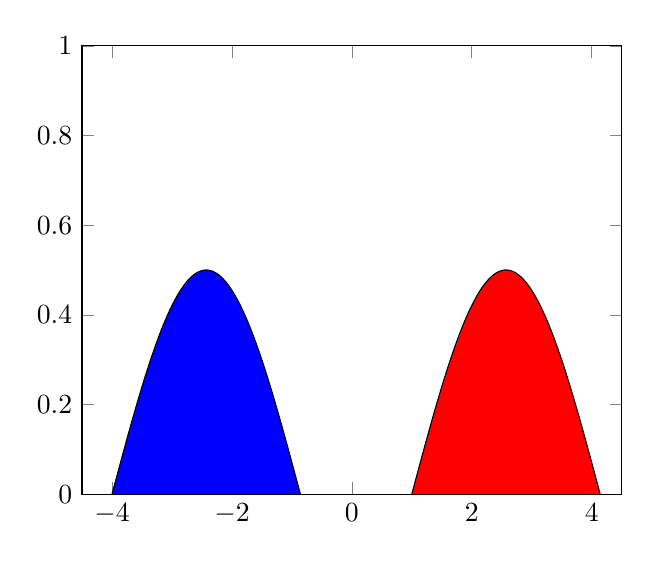
\begin{tikzpicture}
    \begin{axis}[ymin=0, ymax=1, xmin=-4.5, xmax=4.5]
      \addplot[domain=-4:-0.8584,samples=100,fill=blue]{sin(deg(x+4))/2};
      \addplot[domain=1:4.1416,samples=100, fill=red]{sin(deg(x-1))/2};
      \end{axis}
  \end{tikzpicture}
  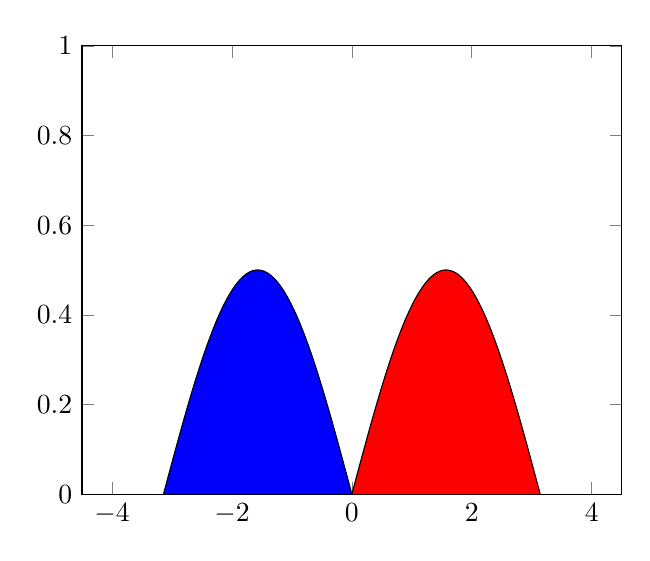
\begin{tikzpicture}
    \begin{axis}[ymin=0, ymax=1, xmin=-4.5, xmax=4.5]
      \addplot[domain=-3.1416:0,samples=100,fill=blue]{sin(deg(x+3.1416))/2};
      \addplot[domain=0:3.1416,samples=100, fill=red]{sin(deg(x))/2};
    \end{axis}
  \end{tikzpicture}
  % \missingfigure{two probability distributions moving closer together but same distance}
  \caption{Example of two different probability distances. 
    Even though the probability distributions of the second plot are closer than the ones on the first plot, they have the same distance in the $L^p$ norm.}
  \label{fig:example-wrong-distance}
\end{figure}

\end{comment}
\subsection{The Kantorovich Distance}
\label{sec:kantoro}
In this section, the Kantorovich Distance is presented as a reasonable and usable metric for measuring the distance between two stochastic processes.
For a gentle introduction to the Kantorovich Distance see \citeasnoun{Deng2009}.
% Note that stochastic processes can be represented as random variables by considering each trajectory as an event.

In the context of stability analysis of stochastic programming problems, it has been shown by \citeasnoun{Dupacova2003} that the Kantorovich functional described below
represents a  `natural and suitable'\footnote{\citeasnoun{Dupacova2003}} distance for measuring stochastic processes.
\begin{definition}[Kantorovich distance]
  Let $\mathbb{P}_1:\Omega_1\rightarrow\mathbb{R}$ and $\mathbb{P}_2:\Omega_1\rightarrow\mathbb{R}$ be probability distributions.
  The \textbf{Kantorovich distance} $D_K(\mathbb{P}_1,\mathbb{P}_2)$ is defined as
  \begin{equation}
    \label{eq:define-infinitedim-kantorovich}
    D_K(\mathbb{P}_1, \mathbb{P}_2) = \inf\limits_{\eta\in\mathcal{M}(\mathbb{P}_1,\mathbb{P}_2)}\left\{\int_{\Omega_1\times\Omega_2}c(\omega_1, \omega_2)d\eta(\omega_1,\omega_2)\right\}
  \end{equation}
  The distance $c$ is a mapping with certain properties, which are specified by \citeasnoun{Dupacova2003}.
  For the purposes of this paper, it suffices to say that any vector norm satisfies these conditions.
Here, $\mathcal{M}(\mathbb{P}_1, \mathbb{P}_2)$ is the space of Borel-measures $\eta$ with marginals $\mathbb{P}_1$ and $\mathbb{P}_2$, meaning that $\eta$ is a probability measure on the space $\Omega_1\times\Omega_2$ with the properties
\begin{equation}
  \label{eq:define-borel-measures}
  \int_{B\times \Omega_2} d\eta(\omega_1,\omega_2) = \mathbb{P}_1(B),\;   \int_{\Omega_1\times B} d\eta(\omega_1,\omega_2) = \mathbb{P}_2(B),\; B \in \mathcal{B}
\end{equation}
where $\mathcal{B}$ is the Borel-$\sigma$-field with respect to $\Omega$.\footnote{For definitions of Borel-measures and Borel-$\sigma$-fields, see for example \citeasnoun{Elstrodt2007}.}
\end{definition}
The Kantorovich distance is only defined as a distance between probability.
The definition is easily extended to random variables and stochastic processes in the following way.
Let $\bs\zeta_1(\Omega_1,\mathfrak{A}_1,\mathbb{P}_1)$ and $\bs\zeta_2(\Omega_2,\mathfrak{A}_2,\mathbb{P}_2)$ be random variables.
For the stochastic optimization problem, the event space is of no interest.
Therefore, it can be assumed, that $\zeta_i = id$.
Note that this is particular to the application to stochastic programming.
The Kantorovich distance between these random variables is then defined as
\begin{equation}
  \label{eq:64}
  D_K(\bs\zeta_1,\bs\zeta_2) = \inf\limits_{\eta\in\mathcal{M}(\mathbb{P}_1,\mathbb{P}_2)}\left\{\int\limits_{\Omega_1\times\Omega_2}c(\zeta(\omega_1),\zeta(\omega_2))d\eta(\omega_1,\omega_2)\right\}.
\end{equation}
Stochastic processes can be measured in the Kantorovich distance by their induced random variables (see remark \ref{remark:stochproc-as-randvar}).
As stated above, the filtration information is discarded in this transformation.
Recently, \citeasnoun{Heitsch2010} have shown that disregarding the filtration information in approximating a stochastic process leads to incorrect results.
To deal with this problem, the use of a filtration distance is advocated.
In this work, the issue of retaining the filtration is solved by postulating the structure of the filtration through a filtration tree.
\paragraph{Kantorovich Distance for finite stochastic processes}
Besides its virtues for the stability analysis (see \citeasnoun{Dupacova2003}), an advantage of the Kantorovich Distance is its simple and intuitive representation for discrete random variables.
Consider two discrete random variables $\bs\zeta(I, p)$ and $\bs\chi(J,q)$ with $I,J\subset\mathbb{N}$ (see remark \ref{remark:discrete-randvar-indexsets}).
Translating the infinite dimensional representation of the metric (\ref{eq:define-infinitedim-kantorovich}) into this framework is straightforward.
The integral over the combination of all possible events of the two stochastic processes is replaced by a sum over a finite set.
The distance $c$ remains unchanged.
The measure $\eta$ in its finite equivalent is a matrix of weights satisfying the same conditions of the marginal probabilities.
These conditions are
\begin{align}
  \label{eq:finitedim-marginals-eta}
  \sum_{i\in I} \eta_{ij} &= q_j\\
  \sum_{j\in J} \eta_{ij} &= p_i.
\end{align}
See figure \ref{fig:finite-kantorovich-illustration} for an illustration of the interpretation of these variables in the case of two-dimensional random variables.
Since in the finite case, the argument of the infimum is a finite sum over variables in a compact domain, the infimum can be replaced by the minimum.
Combining these pieces into the full formulation yields
\begin{equation}
  \label{eq:define-finitedim-Kantorovich}
  D_K(\bs\zeta, \bs\chi) = \min\limits_{\eta}\left\{\sum_{i\in I}\sum_{j\in J}c_{ij} \eta_{ij}\left|\; \sum_{i\in I}\eta_{ij}=q_j,\;\sum_{j\in J}\eta_{ij}=p_i,\;\eta_{ij}\geq 0\right.\right\}.
\end{equation}
with $c_{ij}:=c(\zeta_i,\chi_j)$.
This formulation is a linear program, more specifically a minimum cost flow problem.
This means that solutions are readily available even for large problems using state of the art LP solvers.
The above minimum cost flow problem will be at the heart of the derivations of the following sections, as it will serve as the measure for the quality of approximations to infinite dimensional stochastic processes.
\begin{figure}
  \centering
  \begin{tikzpicture}
    \node [draw,ellipse, fill=red!20] (n1) at (0,0) {$p_1=0.1$};
    \node [draw,ellipse, fill=red!20] (n2) at (5.5,1) {$p_2=0.2$};
    \node [draw,ellipse, fill=red!20] (n3) at (10,7.5) {$p_3=0.1$};
    \node [draw,ellipse, fill=red!20] (n4) at (4.5,5.5) {$p_4=0.2$};
    \node [draw,ellipse, fill=red!20] (n5) at (12,1) {$p_5=0.1$};
    \node [draw,ellipse, fill=red!20] (n6) at (8,5) {$p_6=0.2$};
    \node [draw,ellipse, fill=red!20] (n7) at (0.5,8) {$p_7=0.1$};

    \node [draw,ellipse, fill=blue!20] (m1) at (2.3,3) {$q_1=0.3$};
    \node [draw,ellipse, fill=blue!20] (m2) at (5.5,7.5) {$q_2=0.4$};
    \node [draw,ellipse, fill=blue!20] (m3) at (9,3) {$q_3=0.3$};

    \path [line] (n1) -- node [rectangle, draw,fill=white] (eta11){$\eta_{11}=0.1$} (m1);
    \path [line] (n2) -- node [rectangle, draw,fill=white] (eta21){$\eta_{21}=0.1$} (m1);
    \path [line] (n2) -- node [rectangle, draw,fill=white] (eta23){$\eta_{23}=0.1$} (m3);
    \path [line] (n4) -- node [rectangle, draw,fill=white] (eta41){$\eta_{41}=0.1$} (m1);
    \path [line] (n4) -- node [rectangle, draw,fill=white] (eta42){$\eta_{42}=0.1$} (m2);
    \path [line] (n7) -- node [rectangle, draw,fill=white] (eta72){$\eta_{72}=0.1$} (m2);
    \path [line] (n3) -- node [rectangle, draw,fill=white] (eta32){$\eta_{32}=0.1$} (m2);
    \path [line] (n2) -- node [rectangle, draw,fill=white] (eta21){$\eta_{21}=0.1$} (m1);
    \path [line] (n5) -- node [rectangle, draw,fill=white] (eta53){$\eta_{53}=0.1$} (m3);
    \path [line] (n6) -- node [rectangle, draw,fill=white] (eta63){$\eta_{63}=0.1$} (m3);
    \path [line] (n6) -- node [rectangle, draw,fill=white] (eta62){$\eta_{62}=0.1$} (m2);
    
  \end{tikzpicture}
  \caption{Illustration of the parameters of the Kantorovich Distance. Two discrete probability distributions in $\mathbb{R}^2$ are shown. The position of the nodes represents their value in the 2-dimensional space. The probabilities of the discrete probability distributions $p$ and $q$ are given inside the nodes. The measure $\eta$ can be thought of as describing the flow from the nodes of one distribution to the other.}
  \label{fig:finite-kantorovich-illustration}
\end{figure}
\subsection{Scenario Tree Generation}
\label{sec:scen-tree-generation}
In this section we will briefly state the problem definition for which solutions will be proposed below.

Consider again the multi-stage stochastic programming problem $\mathcal{P}(\hat{\bs\xi})$ from \eqref{eq:genericSP}, governed by a stochastic process $\bs\chi$.
Suppose that $\hat{\bs\xi}$ is either infinite dimensional, or too large to handle in full.
The task is to find a discrete stochastic process $\bs\chi$ that satisfies the following properties.
\begin{enumerate}
\item $\bs\chi$ minimizes the Kantorovich distance $D_K(\hat{\bs\xi},\bs\chi)$.
\item The filtration of $\bs\chi$ is similar to that of $\hat{\bs\xi}$.
\end{enumerate}
In this work, the filtration will not be dealt with explicitly.
See \citeasnoun{Heitsch2010} for an introduction to how this can be done.
Instead, the filtration will be postulated beforehand.
The complexity of a stochastic programming problems, which can be measured by the number of variables in the deterministic equivalent,\footnote{see \citeasnoun{Birge1997} for an overview of deterministic equivalents and other solution methods for stochastic programs} is determined by the filtration tree of the scenario tree $\bs\chi$.

Assume that it is possible to sample from $\hat{\bs\xi}$.
Using Monte-Carlo methods, a set of pairs of scenarios and corresponding probabilities $(\xi_i,p_i)$ can be sampled.
This set of scenarios itself can be considered as a new stochastic process $\bs\xi$ with a discrete probability distribution $p$.
For a sufficiently large number of samples,  $D_K(\bs\xi,\hat{\bs\xi})<\epsilon$ for arbitrary $\epsilon>0$ holds with high probability.
Using the triangle inequality, we have
\begin{equation}
  \label{eq:triangle-montecarlo-kantoro}
  D_K(\bs\chi,\hat{\bs\xi}) \leq  D_K(\bs\chi, \bs\xi) + D_K(\bs\xi,\hat{\bs\xi})< D_K(\bs\chi,\bs\xi)+ \epsilon
\end{equation}
Note that $D_K(\bs\chi,\bs\xi)$ is the Kantorovich distance for two discrete random variables \eqref{eq:define-finitedim-Kantorovich}, and can be solved as a linear program.

The optimal stochastic process $\bs\chi$ minimizes the right hand side of \eqref{eq:triangle-montecarlo-kantoro}.
It is now necessary to define the space that $\bs\chi$ may be chosen from.
As stated above, there exists a bijective mapping between scenario trees and stochastic processes.
Recall the definition of a scenario tree as a triple of a filtration tree $\mathcal{T}$, a mapping $\nu:\mathcal{N}_t\rightarrow\mathbb{R}^d$, and a mapping $q:\mathcal{N}_T\rightarrow\mathbb{R}$.
For the optimization, $\mathcal{T}$ has to be postulated.
A sensible choice for most cases are trees with a constant number of children to each node.
After the filtration tree has been fixed, only the mapping $\nu$ and the probabilities $q$ remain to be optimized.
Note that since the number of nodes in $\mathcal{T}$ is finite, $\nu$ and $q$ can be characterized by finite dimensional real vectors.
The general algorithm will proceed along the steps outlined in algorithm \ref{alg:general}.
\begin{algorithm}
  \label{alg:general}
  \caption{Overall Tree Generation Algorithm}
  \KwIn{Stochastic Process $\hat{\bs\xi}$, filtration tree $\mathcal{T}$}
  \KwOut{Discrete stochastic process satisfying the filtration tree $\mathcal{T}$}
  \BlankLine
  \textbf{Sample} $\bs\xi$ from $\hat{\bs\xi}$\;
  \textbf{Solve} $\underset{\nu,q}{\argmin}\; D_K((\mathcal{T},\nu, q), \bs\xi)$\;
\end{algorithm}

In the literature, especially in \citeasnoun{Heitsch2009} and related papers (\cite{Dupacova2003,Heitsch2003,Heitsch2009a,Heitsch2010}), not the tree structure is fixed beforehand, but instead a given tree is reduced by deleting nodes until a maximum distance $D_K(\bs\xi,\hat{\bs\xi})$ is reached.
We view the approach of fixing the tree structure beforehand is a more sensible assumption for the following reasons.
\begin{itemize}
\item a recursive tree structure makes sense in most applications, as the structure of the decisions to be made is recursive as well.
Consider the operator of the pumped-hydro plant mentioned above.
He faces the same decision at each time step, and his measure of uncertainty for any event happening a certain amount of time into the future is independent of the current situation.
\item the number of scenarios is not determined by the error one will allow but is the other way around: The error is determined by the maximum number of scenarios one can handle computationally.
This number of scenarios will be known beforehand.
As the correlation of using more scenarios and lowering the approximation error is strictly monotonic, there is no reason to use less scenarios than one can handle computationally.
\item For the method described in the papers cited above, it is not obvious how the original tree which is then reduced was constructed in the first place.
\end{itemize}

In the above problem, at least two different definitions of feasible sets for the optimization step of algorithm \ref{alg:general} are possible.
Suppose the scenario tree $(\mathcal{T}, \nu, q)$ is optimized to approximate the discrete stochastic process $\bs\xi$.
Depending on the real-world meaning of $\bs\xi$, different choices of $\nu$ may make sense.
For example, if the underlying stochastic process $\hat{\bs\xi}$, from which $\bs\xi$ was sampled, consists of discrete events like coin tosses, the values of $\nu$ should take on only the values of discrete events.
The mapping $\nu$ should be of the form
\begin{equation}
  \label{eq:65}
  \nu_{DE}:\mathcal{N}_t\rightarrow \xi^t(\Omega)\subset\mathbb{R}^d.
\end{equation}
Trees with such a mapping are referred to as \textbf{discrete-event (DE) trees}.
On the other hand, if the original values stem from a real world process for which intermediate values do in fact make sense, there are no such restrictions:
\begin{equation}
  \label{eq:66}
  \nu_{CE}:\mathcal{N}_t\rightarrow \mathbb{R}^d.
\end{equation}
The latter type of trees is called \textbf{continuous-event (CE) trees}.
A typical example of DE trees are coin tosses and dice rolls, but also events like unit failure in a plant belong to this class.
CE trees can be used for example to model prices and demands.

Discrete- and continuous-event trees lead to different optimization problems for the scenario tree generation.
For discrete-event trees, this is
\begin{equation}
  \label{eq:67}
  \min\limits_{\bs\chi\in \mathcal{S}_{DE}(\mathcal{T},\bs\xi)}D_K(\bs\chi, \bs\xi)
\end{equation}
with
\begin{equation}
  \label{eq:68}
  \mathcal{S}_{DE}(\mathcal{T},\bs\xi) := \left\{\bs\chi \text{ SP}\left|\text{scen. tree of }\bs\chi\text{ is } (\mathcal{T},\nu,q)\text{ with }\nu_n\in\bs\xi(\Omega)\right.\right\}.
\end{equation}
For continuous-event tree, we have
\begin{equation}
  \label{eq:69}
  \mathcal{S}_{CE}(\mathcal{T}) := \left\{\bs\chi\text{ SP}\left|\text{scen. tree of }\bs\chi\text{ is } (\mathcal{T},\nu,q)\right.\right\}.
\end{equation}
Obviously, we have
\begin{equation}
  \label{eq:70}
  \mathcal{S}_{DE}(\mathcal{T},\bs\xi) \subset   \mathcal{S}_{CE}(\mathcal{T}) \;\forall\,\bs\xi
\end{equation}

Since both $\bs\xi(I,p)$ and $\bs\chi(J,q)$ are discrete stochastic processes, the Kantorovich Distance is equivalent to the minimum cost flow problem described above (\ref{eq:define-finitedim-Kantorovich}).
Including this definition yields
\begin{equation}
  \label{eq:symbolic-optimization-with-minflow}
  \min_{\bs\chi\in\mathcal{S}(\mathcal{T},\bs\xi)}\left\{\min_{\eta,q}\left\{\sum_{i\in I}\sum_{j\in J}\eta_{ij}c(\xi_i,\chi_j)\left|\sum_{i\in I}\eta_{ij}=q_j,\;\sum_{j\in J}\eta_{ij}=p_i,\;\eta_{ij}\geq 0\right.\right\}\right\}
\end{equation}
The probability distribution $q$ of $\bs\chi$ is not postulated beforehand, but must be determined as part of the optimization problem.
Note that even though $q$ is not explicitly defined as a probability distribution, the equation
\begin{equation}
  \label{eq:q-schliessbedingung}
  \sum_{j\in J} q_j = 1
\end{equation}
is not necessary, and would in fact be redundant.
The probabilities $p_i$ are known to form a probability distribution. Therefore it holds that
\begin{equation}
  \label{eq:proof-sum-q-redundant}
  1 = \sum_{i\in I}p_i = \sum_{i\in I}\left(\sum_{j\in J}\eta_{ij}\right)=\sum_{j\in J}\left(\sum_{i\in I}\eta_{ij}\right)=\sum_{j\in J} q_j.
\end{equation}
This is an important fact in formulating the optimization problems of the following sections, since introducing this equation would violate the constraint qualifications MFCQ and LICQ.
A constraint qualification is crucial if KKT based optimization algorithms such as interior point methods are to be employed for the solution of the optimization problem \cite{Jongen2004}.

The inner minimization can, of course, be combined with the outer minimization to yield the final formulation
\begin{equation}
  \label{eq:symbolic-optimization-with-minflow2}
  \min_{\chi,\eta,q}\left\{\sum_{i\in I}\sum_{j\in J}\eta_{ij}c(\xi_i,\chi_j)\left|\sum_{i\in I}\eta_{ij}=q_j,\;\sum_{j\in J}\eta_{ij}=p_i,\;\eta_{ij}\geq 0\right.\right\}
\end{equation}
The remainder of this thesis will be dedicated to the solution of this optimization problem.
\begin{comment}
\subsubsection{Tree Feasibility Sets}
\label{sec:tree-feas-sets}
In this section, the two feasibility sets $\mathcal{T}$ for scenario trees used in this paper are discussed.
These are the so called \textbf{discrete-event} trees and \textbf{continuous-event} trees.
The former are the model used in the prominent literature \cite{Dupacova2003} and related papers.
The notion of continuous-event trees is not discussed in any of the cited papers, but will prove to be a powerful concept.

A tree structure can be defined by the number of stages $n_s$ and the number of children (branches) $n_c$ to each node.
For a tree defined in that way, the number of scenarios in this tree (which is the same as the number of leaf nodes) is
\begin{equation}
  \label{eq:number-of-leaf-nodes}
  n_L = n_c^{n_s-1}.
\end{equation}
The number of nodes in the tree can be computed with the formula for the geometric series
\begin{equation}
  \label{eq:number-of-nodes}
  n_N = \frac{1-n_c^{n_s}}{1-n_c}
\end{equation}
\paragraph{Discrete-Event Trees} Consider a study on the robustness of a plane-based mail delivery system to cancellation of flights.
A large database of failures is available that can be used as data to form the initial stochastic process.
The next step is to generate a scenario tree from this data.
In order to evaluate the quality of a scenario tree, a metric for the space of all possible events is necessary.
This discrete space does not have a natural underlying metric space.
The metric must therefore be hand-crafted to fit this purpose.
For each pair of events, a \textbf{dissimilarity measure} must be provided.
Note that the tree generation algorithm will base its decision whether or not to aggregate scenarios o the values of the dissimilarity measure.
The modeling and optimization process therefore starts with this step.

Another specialty of this problem is that generating a tree with values other than those encountered in the original stochastic process would not generate meaningful results.
This places a restriction on the space of allowable solution trees $\mathcal{T}$.
We call this kind of process a ``discrete-event''(DE) stochastic processes, as opposed to ``continuous-event''(CE) stochastic processes, for which intermediate values do make sense such as prices.

The restrictions added by the discrete nature of the value space turn problem (\ref{eq:symbolic-optimization-with-minflow2}) into a \textbf{selection problem}:
\begin{center}
  \textit{From the original set of scenarios, select nodes according to the tree structure, such that the Kantorovich Distance is minimized.}
\end{center}
\todo[inline]{include plot what this means (tikz)}
\paragraph{Continuous-Event Trees} In this section, we will present a novel approach to approximating scenario trees.
While the previous section was concerned with generating scenario trees for discrete underlying event spaces, continuous event spaces are very common.
Obvious examples for stochastic processes with continuous state spaces are prices and demands.

In cases where intermediate values are sensible choices for scenarios, the algorithm described above will sacrifice two possibilities for improvement.
First, notice that the general structure of the problem is still given by the same minimum flow problem (\ref{eq:symbolic-optimization-with-minflow2}).
The difference to the MILP formulation is the set of feasible trees $\mathcal{T}$.
If intermediate values for the states are acceptable, as opposed to only those that were part of the original scenario set, it trivially holds that
\begin{equation}
  \label{eq:T-D-subset-T-C}
  \mathcal{T}_D\subset \mathcal{T}_C,
\end{equation}
where $\mathcal{T}_D$ is the set of feasible DE-trees, and $\mathcal{T}_C$ is the set of feasible trees in the continuous case.
It is therefore obvious, that the Kantorovich Distance for the continuous case must be equal to or lower than that of the discrete case.
This means, that the continuous formulation allows for a tighter approximation.
\end{comment}
% \subsubsection{The Kantorovich Distance in a function space approximation interpretation}

%%% Local Variables:
%%% mode: latex
%%% TeX-master: "da"
%%% End:
